\documentclass[11pt,a4paper]{article}
\usepackage[utf8]{inputenc}
\usepackage[T1]{fontenc}
\usepackage[spanish,es-noquoting]{babel}
\usepackage{amsmath,amssymb}
\usepackage{graphicx}
\usepackage{booktabs}
\usepackage{float}
\usepackage{listings}
\usepackage{xcolor}
\usepackage{caption}
\usepackage[margin=2.4cm]{geometry}
\usepackage{hyperref}
\hypersetup{colorlinks=true,linkcolor=blue!50!black,urlcolor=blue!50!black}

\definecolor{codegray}{gray}{0.95}
\definecolor{commentgreen}{rgb}{0.0,0.5,0.0}
\definecolor{keywordblue}{rgb}{0.0,0.0,0.6}
\definecolor{stringmauve}{rgb}{0.58,0.0,0.82}
\lstset{
  language=Matlab, basicstyle=\ttfamily\footnotesize,
  backgroundcolor=\color{codegray}, commentstyle=\color{commentgreen}\itshape,
  keywordstyle=\color{keywordblue}\bfseries, stringstyle=\color{stringmauve},
  numbers=left, numberstyle=\tiny\color{gray}, numbersep=6pt,
  frame=single, rulecolor=\color{gray!40}, breaklines=true,
  columns=fullflexible, showstringspaces=false, captionpos=b,
  xleftmargin=14pt, framexleftmargin=14pt
}
\newcommand{\code}[1]{\texttt{\small #1}}

\begin{document}

% ================= DATOS =================
\section{Datos generales}
\begin{center}
\renewcommand{\arraystretch}{1.3}
\begin{tabular}{ll}
\toprule
\textbf{Curso} & Inteligencia Artificial Aplicada al Control (ICA636-0001) \\
\textbf{Trabajo} & Tarea 6 --- Lógica Difusa \\
\textbf{Alumno} & Joel Arzapalo Guerra \\
\textbf{Código} & 20032006 \\
\textbf{Fecha} & \today \\
\bottomrule
\end{tabular}
\end{center}
\vspace{0.4cm}

% ================= INTRODUCCION =================
\section{Introducción}
Este trabajo analiza dos controladores de \textbf{lógica difusa} para robots móviles
(Clases 11--13): un robot \textbf{tipo carro} (\code{fuzzycarxloco.m}) y un robot
\textbf{tipo trailer} (\code{fuzzytrailerxbueno.m}). Ambos calculan el ángulo del timón
$\delta$ a partir de la posición y la orientación del vehículo mediante un sistema difuso
de tipo Mamdani. El trabajo tiene dos partes:
\begin{enumerate}
  \item \textbf{Revisar y mejorar la tabla de reglas} del carro (\code{fuzzycarxloco.m}):
        la base de reglas original produce un control brusco y no siempre estaciona; se
        rediseña para lograr un control suave y convergente.
  \item \textbf{Adaptar el trailer} (\code{fuzzytrailerxbueno.m}) para que alcance
        $y^*=50$ en lugar de $x^*=50$: se rota el problema $90^\circ$ de modo que el
        difuso regule la coordenada $Y$ hacia $50$ mientras el vehículo avanza en $+x$.
\end{enumerate}
Para evaluar los cambios de forma reproducible, los scripts (interactivos, con
\code{input()} y animación) se adaptaron a versiones no interactivas
(\code{fuzzycar\_sim.m}, \code{fuzzytrailer\_sim.m}) que conservan exactamente la
inferencia difusa original y devuelven la trayectoria.

% ================= ANALISIS DE CODIGO =================
\section{Análisis del código}

\subsection{Estructura del controlador difuso}
Ambos controladores siguen el esquema Mamdani clásico con tres etapas:
\begin{itemize}
  \item \textbf{Fuzzificación:} cada variable de entrada (posición $X$, orientación
        $\phi$; en el trailer además el ángulo de articulación $\theta_{12}$) se parte en
        7 conjuntos difusos triangulares con traslape, y se calcula el grado de
        pertenencia de la medición a cada uno.
  \item \textbf{Base de reglas:} una matriz \code{BaseReg} indexada por las regiones
        activas de las entradas devuelve la región del timón $\delta$ (1=NB\dots7=PB). El
        grado de activación de cada regla es el mínimo de las pertenencias (operador AND).
  \item \textbf{Defuzzificación:} se agregan las salidas por \emph{máximo} sobre el
        universo de $\delta$ y se calcula el \textbf{centroide} (centro de área), que da
        el valor nítido de $\delta$.
\end{itemize}
Las 7 particiones son: para $X$ (posición relativa a la meta) LE, LEC, LC, \textbf{CE}
(centro), RC, RIC, RI; para $\phi$ RB, RU, RV, \textbf{VE} (vertical), LV, LU, LB; para
$\delta$ NB, NM, NS, \textbf{ZE}, PS, PM, PB (negativo grande $\to$ positivo grande).

\subsection{Robot tipo carro}
El vehículo sigue el modelo bicicleta $\phi_{k+1}=\phi_k-\tfrac{r}{L}\tan\delta$,
$x_{k+1}=x_k+r\cos\phi$, $y_{k+1}=y_k+r\sin\phi$. La meta es estacionar en $x=x_{des}$
con orientación \emph{vertical} ($\phi=90^\circ$), moviéndose hacia arriba hasta $y>100$.
La posición se centra con \code{xnuevo = x + 50 - xdeseado} (así $x=x_{des}$ corresponde
al conjunto central CE en $50$).

\subsection{Robot tipo trailer}
El trailer añade el ángulo de articulación $\theta_{12}$ (tercera entrada difusa, 3
conjuntos) y una tabla de reglas \textbf{tridimensional}. Su cinemática articulada es
\[
  \dot\theta_2=-\tfrac{v}{L_2}\sin\theta_{12},\quad
  \dot\theta_{12}=\tfrac{v}{L_2}\sin\theta_{12}-\tfrac{v}{L_1}\tan\delta,\quad
  \dot x=v\cos\theta_{12}\cos\theta_2,\quad \dot y=v\cos\theta_{12}\sin\theta_2 .
\]
Al igual que el carro, regula la coordenada $X$ del trailer hacia $x_{des}$ mientras
avanza hacia arriba.

% ================= PARTE 1 =================
\section{Parte 1: mejora de la tabla de reglas del carro}
\label{sec:car}

\subsection{Problema de la tabla original}
La base de reglas original solo usa \textbf{tres} de los siete valores de timón
—NB (1), ZE (4) y PB (7)—, es decir un control muy brusco (usa casi solo los valores
extremos del timón), y varias de sus
filas son incoherentes:
\[
\text{BaseReg}_{\text{orig}}=
\begin{bmatrix}
1&1&1&4&7&7&7\\
1&1&1&4&7&7&7\\
1&7&7&4&7&7&1\\
7&7&7&4&7&7&1\\
1&7&7&4&7&7&1\\
1&1&1&4&7&7&7\\
1&1&1&4&7&7&7
\end{bmatrix}
\]
El defecto más grave está en la fila \textbf{VE} (vehículo vertical): asigna PB
(girar a la derecha) en casi todas las columnas, incluso cuando el carro ya está a la
\emph{derecha} del centro (columnas RC, RIC), donde debería girar a la izquierda. Además
las filas RV/LV alternan NB y PB en columnas contiguas (control errático). El resultado
es un timón que cambia bruscamente y trayectorias con lazos que no siempre estacionan
(Fig.~\ref{fig:cartraj}, izquierda).

\subsection{Tabla de reglas mejorada}
Se rediseñó la tabla con los \textbf{siete} niveles de timón, siguiendo la ley
$\delta \propto (\phi-\phi^*)$ con una orientación deseada
$\phi^*=90^\circ + K\,(x-x_{des})$: si el carro está a la izquierda del centro debe
apuntar un poco a la derecha ($\phi^*<90$), y viceversa. Discretizando esa ley se obtiene
una tabla \textbf{graduada, monótona y simétrica}:
\[
\text{BaseReg}_{\text{nueva}}=
\begin{bmatrix}
1&1&1&1&1&1&1\\
2&1&1&1&1&1&1\\
6&4&3&2&2&1&1\\
7&6&5&4&3&2&1\\
7&7&6&6&5&4&2\\
7&7&7&7&7&7&6\\
7&7&7&7&7&7&7
\end{bmatrix}
\]
La fila central VE ahora es $[7\,6\,5\,4\,3\,2\,1]$: a la izquierda del centro gira a la
derecha de forma proporcional, en el centro va recto (ZE) y a la derecha gira a la
izquierda, que es el comportamiento correcto de auto-centrado.

\subsection{Resultados}
Se compararon ambas tablas estacionando en $x_{des}=50$ desde cuatro condiciones
iniciales. La tabla mejorada convierte las trayectorias con lazos de la original en
\textbf{aproximaciones suaves} a la recta $x=50$ (Fig.~\ref{fig:cartraj}), y reduce tanto
el error final como la aspereza del timón (Tabla~\ref{tab:car}, Fig.~\ref{fig:cardelta}):
el error de posición final medio baja de $15.0$ a $3.4$ y la variación total del timón
(medida de brusquedad) de $387$ a $74$.

\begin{table}[H]\centering
\caption{Comparación tabla original vs mejorada (error final en $x$ y variación total del
timón, TV; menor es mejor).}
\label{tab:car}
\begin{tabular}{lcccc}
\toprule
 & \multicolumn{2}{c}{Original} & \multicolumn{2}{c}{Mejorada} \\
Condición inicial & error $x$ & TV($\delta$) & error $x$ & TV($\delta$) \\
\midrule
$x_0{=}20,\ \phi_0{=}90^\circ$  & 2.25  & 547 & 2.09 & 81 \\
$x_0{=}80,\ \phi_0{=}90^\circ$  & 29.96 & 600 & 2.09 & 81 \\
$x_0{=}30,\ \phi_0{=}135^\circ$ & 7.48  & 400 & 4.75 & 68 \\
$x_0{=}70,\ \phi_0{=}45^\circ$  & 20.38 & 0   & 4.75 & 68 \\
\midrule
\textbf{Media} & \textbf{15.0} & \textbf{387} & \textbf{3.4} & \textbf{74} \\
\bottomrule
\end{tabular}
\end{table}

\begin{figure}[H]
\centering
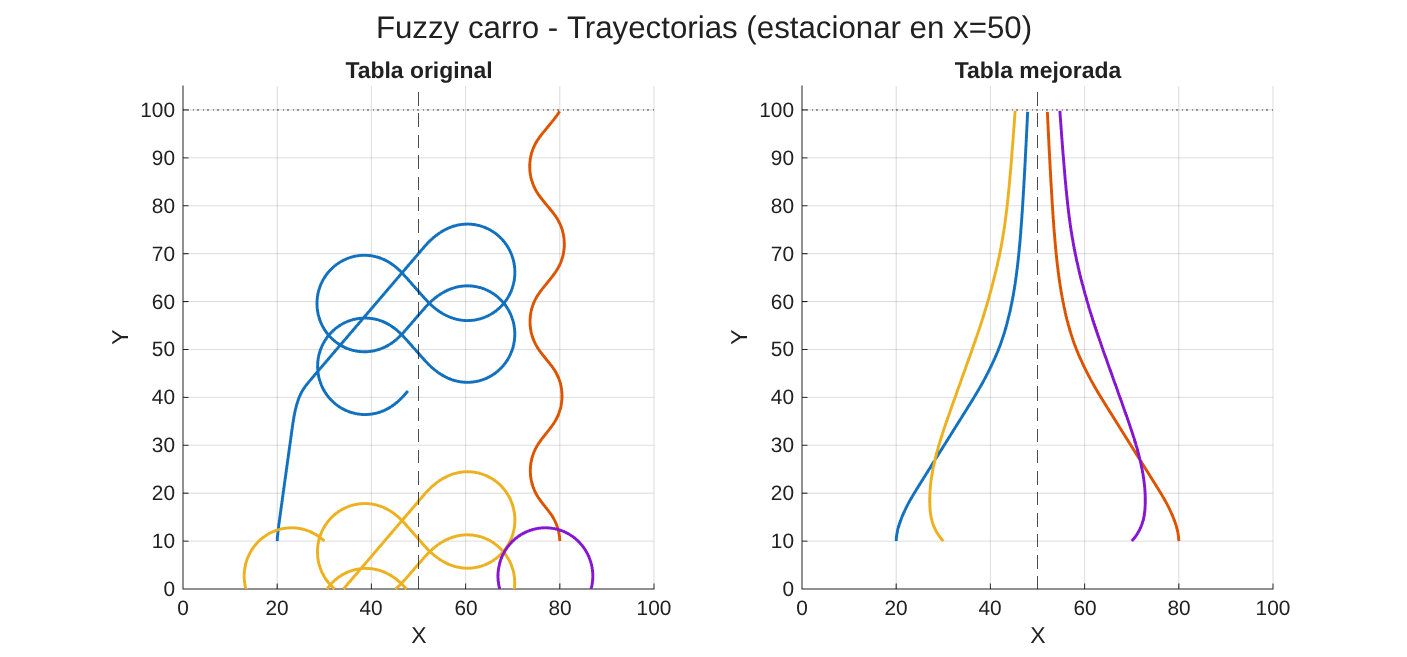
\includegraphics[width=0.95\linewidth]{figs/car_traj.png}
\caption{Trayectorias del carro difuso (estacionar en $x=50$). Izquierda: tabla original
(lazos, no siempre estaciona). Derecha: tabla mejorada (convergencia suave).}
\label{fig:cartraj}
\end{figure}

\begin{figure}[H]
\centering
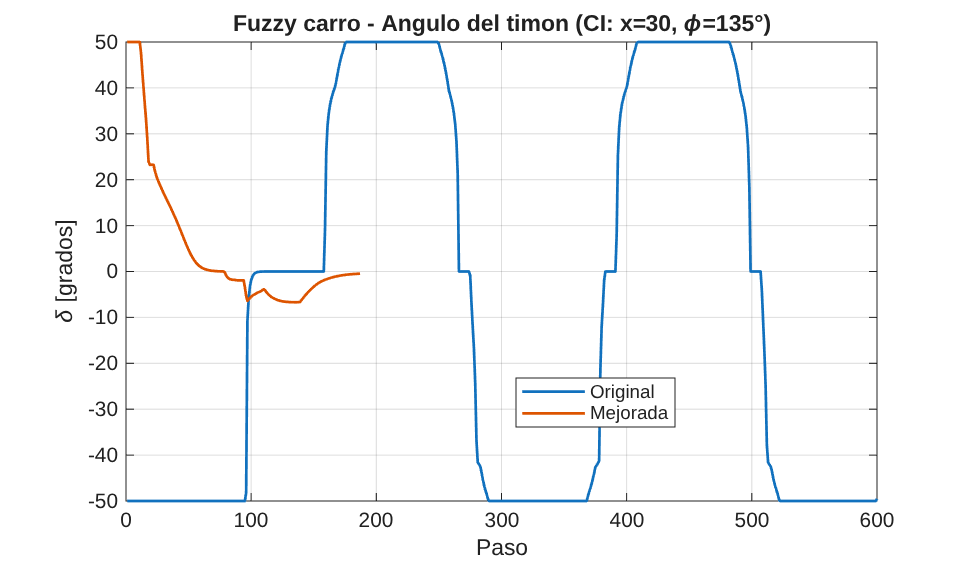
\includegraphics[width=0.6\linewidth]{figs/car_delta.png}
\caption{Ángulo del timón: la tabla original oscila bruscamente; la mejorada es suave.}
\label{fig:cardelta}
\end{figure}

% ================= PARTE 2 =================
\section{Parte 2: el trailer alcanza $y^*=50$}
\label{sec:trailer}
El controlador original regula la coordenada $X$ del trailer hacia $x_{des}$ mientras el
vehículo avanza hacia arriba (orientación objetivo $\theta_2=90^\circ$) hasta $y>100$. Se
pide que en cambio alcance $y^*=50$.

\subsection{Rotación del problema $90^\circ$}
En lugar de reescribir la inferencia, se \emph{rota} el problema: la variable de posición
del difuso se alimenta con la coordenada $Y$ y la de orientación con
$\theta_2+90^\circ$, de modo que el vehículo avance en $+x$ y regule $y$ hacia $50$. Las
sustituciones son:
\[
  \text{posición:}\quad \text{posvar}=50+y_{des}-y \quad(\text{en vez de } x+50-x_{des}),
  \qquad
  \text{orientación:}\quad \phi_{fz}=\theta_2+90^\circ ,
\]
y la condición de término pasa a ser $x>100$. Así $\theta_2=0^\circ$ (avanzar al este)
corresponde al conjunto ``vertical'' del difuso, y $y=y_{des}$ al conjunto central. La
\textbf{cinemática y la tabla de reglas 3D no cambian}. Fue necesario ampliar la
\emph{normalización angular} de $\theta_2$ a $(-180^\circ,180^\circ]$ para el caso rotado (el
original lo mantenía cerca de $90^\circ$ y dejaba al vehículo sin control al girar hacia
abajo).

\subsection{Resultados}
Partiendo de cuatro posiciones iniciales por encima y por debajo de la meta
($y_0=20,80,35,65$, con $\theta_2=0^\circ$), el trailer \textbf{alcanza y sigue la recta
$y=50$} y avanza hasta $x=100$ (Fig.~\ref{fig:trailery}); los valores finales de $y$ son
$50.1,\ 49.9,\ 50.1,\ 49.9$. La Fig.~\ref{fig:trailerst} muestra que la orientación del
remolque $\theta_2$ tiende a $0^\circ$ (horizontal), el ángulo de articulación
$\theta_{12}$ se estabiliza y el timón $\delta$ se aquieta al llegar a la recta objetivo.

\begin{figure}[H]
\centering
\begin{minipage}{0.55\linewidth}\centering
  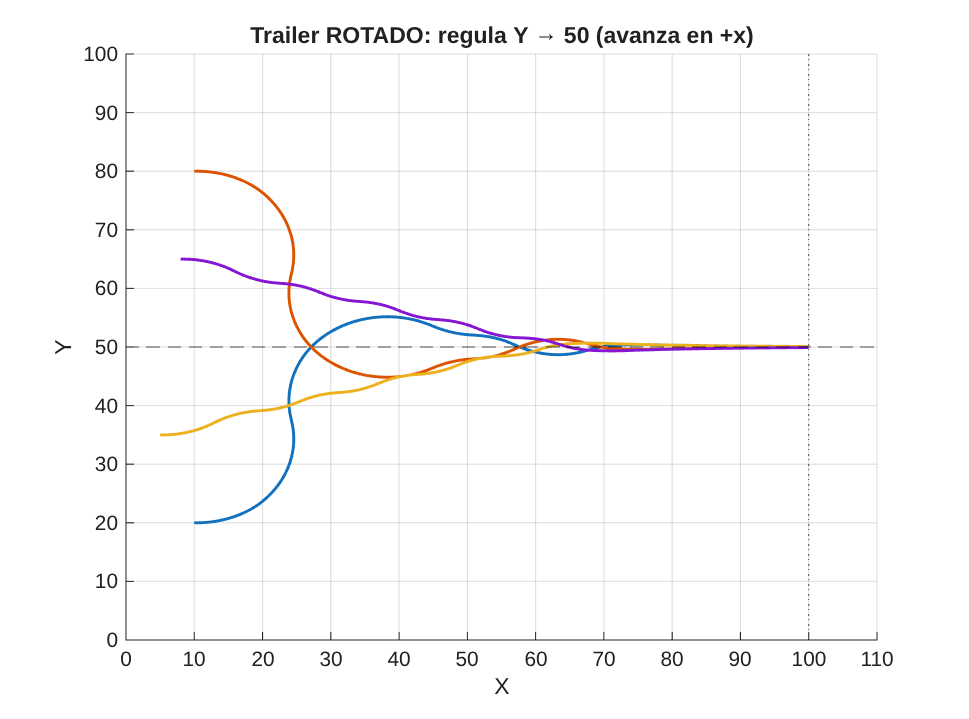
\includegraphics[width=\linewidth]{figs/trailer_y.png}
  \caption{Trailer rotado: regula $Y\to50$ desde CI por encima y por debajo.}
  \label{fig:trailery}
\end{minipage}\hfill
\begin{minipage}{0.43\linewidth}\centering
  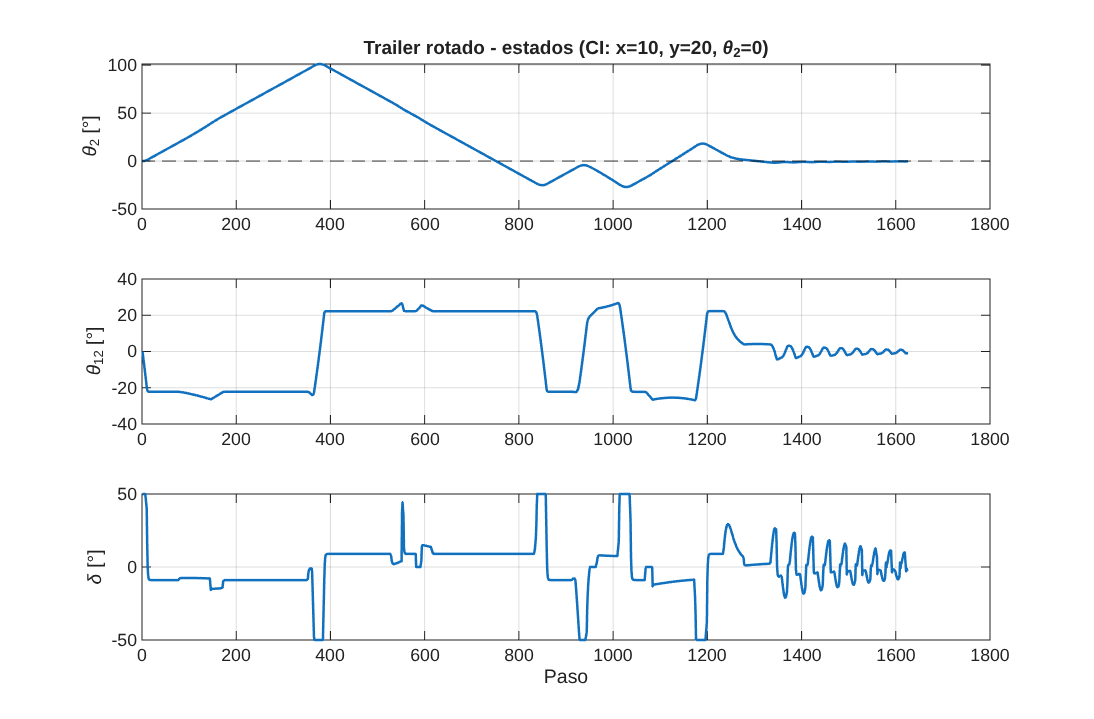
\includegraphics[width=\linewidth]{figs/trailer_y_states.png}
  \caption{Estados $\theta_2,\theta_{12},\delta$.}
  \label{fig:trailerst}
\end{minipage}
\end{figure}

% ================= CONCLUSIONES =================
\section{Conclusiones}
\begin{enumerate}
  \item \textbf{La tabla de reglas es el corazón del control difuso} (Sec.~\ref{sec:car}).
  La tabla original del carro, al usar solo tres niveles de timón y tener filas
  incoherentes, generaba un control brusco que no siempre estacionaba. Rediseñarla con los
  siete niveles siguiendo una regla clara —girar en proporción al error de orientación
  deseado— produjo trayectorias suaves y convergentes, reduciendo el error final medio de
  $15.0$ a $3.4$ y la brusquedad del timón cinco veces.

  \item \textbf{Un buen diseño de reglas es más importante que el ajuste fino:} bastó una
  tabla graduada, monótona y simétrica para transformar por completo el comportamiento,
  sin tocar las funciones de pertenencia ni la defuzzificación.

  \item \textbf{El mismo controlador sirve para una meta distinta} (Sec.~\ref{sec:trailer}).
  Rotando el problema $90^\circ$ —alimentando la posición con $Y$ y la orientación con
  $\theta_2+90^\circ$— el trailer alcanza $y^*=50$ en lugar de $x^*=50$, sin modificar la
  cinemática ni la base de reglas: solo cambian las entradas al sistema difuso y la
  condición de término.
\end{enumerate}

\appendix
\section{Archivos del proyecto}
Los experimentos se ejecutan con \code{Informe/exp/}: \code{fuzzycar\_sim.m} y
\code{car\_experiments.m} (carro, tabla original vs mejorada) y
\code{fuzzytrailer\_sim.m} con \code{trailer\_experiments.m} (trailer, modos $X$ e $Y$).
Son versiones no interactivas de \code{fuzzycarxloco.m} y \code{fuzzytrailerxbueno.m} que
conservan la inferencia difusa original.

\end{document}
